%\documentclass{article}
\documentclass{proc}

\usepackage[margin=2.54 cm]{geometry}

%Package for working with graphics
\usepackage{graphicx}

\title{Including Graphics}
\author{Chris Jaime}
\date{}



\begin{document}

\maketitle

\section{Introduction}

Picture books are just \emph{better}.

\subsection{Including graphics}

This is a banana in a JPG.

\vspace{0.5cm} %Add some vertical space

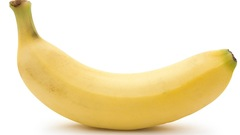
\includegraphics[scale=0.5]{Banana.jpg}

This is a fish, in a chart, in a PNG.

\vspace{0.5cm} %Add some vertical space

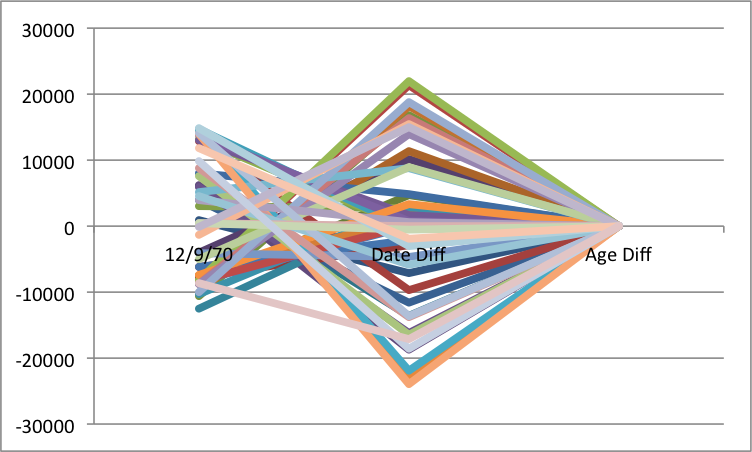
\includegraphics[scale=0.5]{Fish.png}

\subsection{Float: Figure Environment}
In my article, I want to include a JPG image of a banana. You can see this image in the Figure~\ref{fig:banana}.

\begin{figure}[htbp]
	\begin{center}
	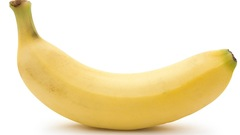
\includegraphics[scale=0.5]{Banana.jpg}
	\caption{This is a banana}
	\label{fig:banana}
	\end{center}
\end{figure}

In my article, I want to include a PNG image of a chart that looks like a fish. You can see this image in the Figure~\ref{fig:fish}.

\begin{figure}[htbp]
	\begin{center}
	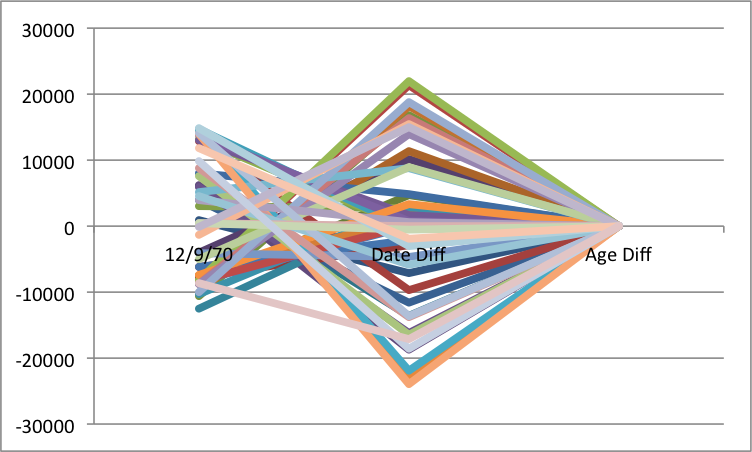
\includegraphics[width=5 cm]{Fish.png}
	\caption{This is a chart that looks like a fish.}
	\label{fig:fish}
	\end{center}
\end{figure}


\section{Conclusion}
Adding images to an article.

\end{document}

 